\documentclass[conference]{IEEEtran}

\usepackage{cite}
\usepackage{algorithm2e}


\ifCLASSINFOpdf
 \usepackage[pdftex]{graphicx}
 \graphicspath{{pics/}}
 \DeclareGraphicsExtensions{.pdf,.jpeg,.png}
\fi
 
\begin{document}
\title{Solving complex reliability networks using conditional probability.}

\author{\IEEEauthorblockN{Anthony Yaghi}
\IEEEauthorblockA{School of Electrical and Computer Engineering\\
Lebanese American University\\
Lebanon, Byblos\\
Email: anthony.yaghi@lau.edu}
}

\maketitle

\begin{abstract}

\end{abstract}

\section{Introduction}
The field of reliability study started to take shape during the second world
war. A lot of new military equipment were introduced and the main application
of reliability study was focused on the vacuum tube which was an integral part of many
of these equipment, like radar systems. And so, the military needed a
measurement of how likely these costly equipment were to fails in order to
mitigate the risk of a malfunction during the war. Today, reliability study
is a large field with both military and commercial applications. A common way to
represent a system is using a graph or a network where each edge represents a
component, by using this representation, one can visualize the system which
makes it easier to apply different evaluation methods. One such evaluation
method is the conditional probability approach, it consists of simplifying the
system by reducing it into a set of series-parallel systems and re-combining
their solution. The conditional probability approach is a very powerful tool
that can be used to solve any complex system elegantly; in this project we will
explore the possibility of implementing this method on a computer. The objective
is to have a working implementation that is capable of taking a representation
of a system and finding the best way to reduce it using the conditional probability
approach. In addition, the implementation could be used as an educational tool
to show visually how a system gets divided into 2 new sub-systems for a given
component. We will start by explaining the conditional probability
method and how to transform it into an algorithm. In the second part of the
report, we will present the actual implementation and the technical challenges
faced. Finally, we will see how the implementation will perform on a set of
different problems/networks.\\

\section{The Conditional Probability Approach}
\subsection{Method}
The conditional probability approach consists of gradually breaking a complex
system into smaller and simpler series-parallel sub-systems. The reliability of
the original system can then be obtained by combining the solutions of the
sub-systems using conditional probability, hence the name. Take for example the
following network of components.\\
\begin{figure}[h]
  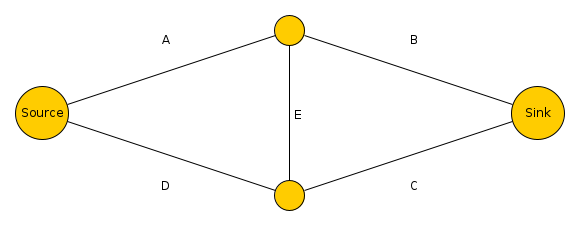
\includegraphics[scale=0.5]{demo_sys_1}
  \label{fig:sys1}
\end{figure}
\\
It can be reduced into 2 sub-systems each of which is a series-parallel system.\\
\begin{figure}[h]
  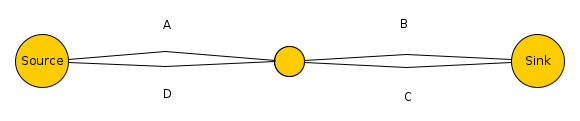
\includegraphics[scale=0.5]{demo_sys_1_e_good}
  \caption{E is good}
  \label{fig:egood}
\end{figure}
\\
\begin{figure}[h]
  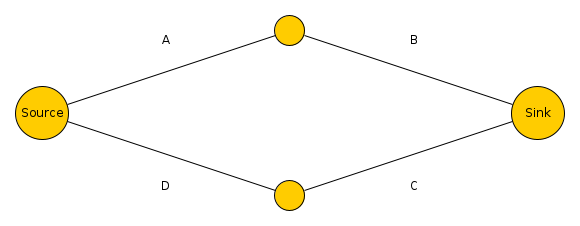
\includegraphics[scale=0.5]{demo_sys_1_e_bad}
  \caption{E is bad}
  \label{fig:ebad}
\end{figure}
\\
Figure \ref{fig:egood} shows the resulting network when we take component E to
be always good. Figure \ref{fig:ebad} on the other hand, shows the network when
we take component E to be bad. The reliability of the original system can be
then written as\\
$R_{sys} = R_E \times R_{sub-sys1} + Q_E \times R_{sub-sys2}$\\
Where $Q_E = 1 - R_E$, $sub-sys1$: when E is good and $sub-sys2$: when E is bad.
All that is left to do is solve $R_{sub-sys1}$ and $R_{sub-sys2}$ which is a
trivial task since both are series-parallel. For more complex systems, breaking
it down once will not necessarily lead immediately to 2 series-parallel
sub-systems. In this case, the process should be repeated on the resulting
sub-systems until we end up with only series-parallel networks that can be
easily solved.
\subsection{Algorithm}
In this section I will propose an algorithm to find all the possible ways a
system can be reduced in, then search for the smallest/fastest combination of
components that will reduce it to a set of series-parallel systems. The method
described above can be implemented cleanly by building a tree, where each node
is a graphs, recursively. A graph represents a system where each component is an
edge, so in what follows I will be using the word graph instead of system.\\
The idea is to start with the main graph as the root of the tree and expand tree
with 2 branches for each component in the graph. One branch will lead to a node
where the component is good and the other to a node where it is bad. Each child
node is then expanded in turn recursively. The algorithm stops expanding a
branch when a series-parallel graph is reached.

\begin{algorithm}
\SetAlgoLined
\SetKwFunction{FMain}{BuildTree}
\SetKwProg{Fn}{Function}{:}{}
\SetKw{new}{new}
\SetKw{reduce}{reduce}
\SetKw{good}{good}
\SetKw{bad}{bad}

\KwIn{node containing a reliability graph}
\KwOut{Conditional probability tree}
\BlankLine

\Fn{\FMain{$root$}}{
  \uIf{$root$ is series-parallel}{
    \Return{}\;
  }
  \Else{
    $graph \leftarrow root.data$\;
    \For{$edge \in graph$}{
      $goodNode \leftarrow$ \new $node$\;
      $badNode \leftarrow$ \new $node$\;
      $goodGraph \leftarrow \reduce(graph, edge, \good)$\;
      $badGraph \leftarrow \reduce(graph, edge, \bad)$\;
      $goodNode.data \leftarrow goodGraph$\;
      $badNode.data \leftarrow badGraph$\;
      \BlankLine
      \FMain{$goodNode$}\;
      \FMain{$badNode$}\;
      \BlankLine
      $root.addChild(goodNode)$\;
      $root.addChidl(badNode)$\;
      \Return{}
    }
  }
}
\caption{Algorithm for building the conditional probability tree}
\label{alg:buildTree}
\end{algorithm}

Once the tree is built it is now possible to find the smallest combination of
edges/components needed to reduce the system into a set of series-parallel
graphs. A depth first search will go over the previously built tree and give a
weight to every branch equal to the depth of the sub-tree connected to it. The
next  step will be to simply cut all the branches at the first level except the
pair with the smallest combined weight. Notice that in algorithm
\ref{alg:buildTree} each edge in the graph will lead to the creation of 2 nodes
and thus 2 branches. It is crucial in this step to consider these pair of
branches together otherwise the logic will be false. This means that there is a
single combined score for each pair and if one branch is removed the other one
should be removed as well.

\begin{algorithm}
\SetAlgoLined
\SetKwFunction{FMain}{FindWeights}
\SetKwProg{Fn}{Function}{:}{}

\KwIn{root node of a tree}
\BlankLine

\Fn{\FMain{$root$}}{
  \uIf{$root.branches = \emptyset$}{
    \Return{0}\;
  }
  \Else{
    \For{$branch \in root.branches$}{
      $w = \FMain{branch.node}$\;
      $branch.weight = w + 1$\;
    }
  }
}
\caption{Algorithm for finding branches weights}
\label{alg:addWeights}
\end{algorithm}

\section{Implementation and challenges}
\subsection{Programming language and packages}
In order to implement the algorithms proposed above we should be able to easily
represent graphs and do operations on the nodes and edges, in the code. For this
reason NetworkX \cite{networkx}, a python package, was used. NetworkX allows the
creation of many type of graphs, for this implementation a MultiGraph is used.
It is a type of graph with undirected edges and which allows more than 1 edge
between 2 nodes. This is an important property otherwise it will be impossible
to have parallel edges/components. A graph is a list of nodes connected by a
list of edges, by using NetworkX a single method can add a whole list of nodes
or edges. In addition to be able to create graphs, this packages offers a range
of algorithms from graph theory that can be directly used.\\
Drawing graphs was done using Matplotlib, 'Matplotlib is a Python 2D plotting
library which produces publication quality figures in a variety of hardcopy
formats and interactive environments across platforms.'\cite{matplotlib}

\subsection{Series-parallel graphs}
One of the main challenges of this project was to find a good way to tell if a
given graph is in a series-parallel configuration. There are many definition for
a SP-graph in the literature, but I ended up adopting the definition introduced
by Duffin, R.J.\cite{spg}. First the graph should have 2 distinguished nodes,
the source and the sink, labeled $s$ and $t$. Such a graph is a SP-graph if it can be
reduces to a $K_2$ using the following operations:
\begin{enumerate}
\item{Replace 2 edges connected by a node with degree 2, other than $s$ or $t$, by 1 edge}
\item{Replace 2 edges that are parallel by 1 edge}
\end{enumerate}
A $K_n$ graph is a graph having $n$ nodes where each pair of nodes is connected
by a unique edge. In our case, this means that a $K_2$ graph is a graph with a single edge
connecting the source and sink nodes.

\subsection{Detecting shorted components}
Assuming a component to be good will reduced the graph and can lead to having
one or multiple components shorted. Since this operation is carried out
multiple times when building the conditional probability tree, it was important
to find a way to detect and eliminate these shorted components. In graph theory
a loop is a list of edges that connect a node back to itself. Based on this
definition, we can detect a series of shorted components/edges by finding a loop
that contains only nodes of degree 2, except the origin node which can have any
degree. Once such a loop is found, the algorithm will remove all the edges that
forms the loop, then check for any nodes with degree 0 and remove them as well.
This step should be perform each time a graph is reduced by considering a node
to be always good.


\section{Conclusion}
The conclusion goes here.


\bibliographystyle{IEEEtran}
\bibliography{refs}

\end{document}
% LocalWords:  Yaghi edu sys NetworkX FindWeights NetworkX MultiGraph undirected
% LocalWords:  Matplotlib hardcopy
